%!TEX program = xelatex
\documentclass[titlepage,oneside]{ctexart}
\usepackage{ecustpc} % 加载刚才定义的样式

% 定义竞赛信息
\title{2026年华东理工大学程序设计锦标赛试题册}
\author{ECUSTPC 2026 Spring Jury}
\date{April 7th, 2026}

\begin{document}

% 设置页眉内容：竞赛名称，日期
\setcontestheader{2026 年华东理工大学程序设计锦标赛 正式赛}{2026年4月7日}
\pagestyle{fancy}

\setlength{\headheight}{25.3186pt}

\begin{titlepage}
\begin{center}
    \huge{\textbf{2026 年华东理工大学程序设计锦标赛}} \\ [10pt]
    \huge{正式赛 \quad 试题册} \\ [10pt]
    \Large{2026 年 4 月 7 日 12:30 $\sim$ 17:30}
\end{center}    

\vspace{2em}
{\large\BF{试题列表}}

\begin{table}[htbp]
  \begin{center}
    \large
    \begin{tabular}{ccccc}
      \toprule
      题号 & 试题名称 & 时空限制 & 注释 \\
      \midrule
      \myboxi{\BF{\TT{A}}} & \BF{聚光灯下} & 5s/1GB & \\
      \myboxii{\BF{\TT{B}}} & \BF{回响形态} & 1s/1GB & \\
      \myboxiii{\BF{\TT{C}}} & \BF{星之所在} & 1s/1GB & \\
      \myboxiv{\BF{\TT{D}}} & \BF{左灯右行} & 1s/1GB & 交互题 \\ 
      \myboxv{\BF{\TT{E}}} & \BF{右灯左行} & 1s/1GB & \\
      \myboxvi{\BF{\TT{F}}} & \BF{迷路日} & 1s/1GB & \\ 
      \myboxvii{\BF{\TT{G}}} & \BF{朝复习} & 1s/1GB & \\
      \myboxviii{\BF{\TT{H}}} & \BF{朝复夕} & 2s/1GB & \\
      \myboxix{\BF{\TT{I}}} & \BF{星露谷物语} & 1s/1GB & \\
      \myboxx{\BF{\TT{J}}} & \BF{烈焰风暴 2} & 1s/1GB & \\
      \myboxxi{\BF{\TT{K}}} & \BF{净化行动 2} & 2s/1GB & \\
      \myboxxii{\BF{\TT{L}}} & \BF{海底捞月} & 2s/1GB & \\
      \bottomrule       
    \end{tabular}
  \end{center}
\end{table}

试题册共包含 12 道试题和 21 页.

若您的试题册缺页请立刻联系志愿者。

请务必认真阅读位于比赛文件附件中的赛事规则和技术规则。

赛事开始前请勿翻阅试题册，亦请勿触碰鼠标和键盘。

请注意黑白打印的试题册可能会丢失部分需要颜色展现的信息。

\textit{写在题目描述前的斜体文字 是 Feature Text（风味文本），和题目无关，包括这句话。}
\end{titlepage}

\linespread{1.0}
\setlength{\parskip}{0\baselineskip}
\normalsize

\newpage
\setcounter{page}{1}

% 引入题目文件 (建议将题目放在子目录中)
% \input{problems/A}
% \newpage
% \input{problems/B}
\section[A. 聚光灯下]{\myboxi{      \BF{\TT{A}}} 聚光灯下}

\textit{运行时间限制}   5 seconds

\textit{内存使用限制} 1 Gigabyte

\textit{读入文件} \qquad 标准输入

\textit{输出文件} \qquad 标准输出


\begin{quote}
	\textit{当猩红的幕布被缓缓拉开，你便再没有退路。\\
哪怕台下坐着的是漫天神佛，是不可名状的灾厄……\\
只要你还站在台上，这场戏，就必须演到落幕。}
\end{quote}

\subsection{题目描述}

Bean 安置的舞台即将开始美妙的表演 ...

舞台是一个二维欧几里得平面，小人 A 初始站在舞台中心，也即坐标原点 $(0, 0)$. 舞台上方有 $n$ 盏聚光灯，每盏聚光灯会在平面上打出一个以 $(x_i, y_i)$ 为圆心，半径为 $\sqrt{x_i^2 + y_i^2}$ 的圆形光照区，圆形边界也在光照区内，可以发现舞台中心在所有聚光灯的光照区内。

为展现表演的张力，A 希望在表演的移动途中始终在每一盏聚光灯的光照区内，并走到距离舞台中心最远的点。

请帮助 A 求出她在移动轨迹不离开任何一盏聚光灯的光照区的条件下，能走到最远的点到舞台中心的距离。

\subsection{输入格式}

第一行输入一个整数 $T$ ($1 \le T \le 10^5$), 表示测试数据的数量。

每组测试数据第一行输入一个整数 $n$ $(1 \le n \le 10^5)$, 表示聚光灯的数量。

随后 $n$ 行输入两个整数 $x_i$ 和 $y_i$ ($-10^5 \le x_i, y_i \le 10^5$, $(x_i, y_i)$ 不和原点重合)，表示一盏聚光灯的光照区中心。

保证所有测试数据的 $\sum n \le 3 \times 10^5$.

保证单组测试数据中任意两个聚光灯的光照区中心不同，任意三个聚光灯的中心区不共线。

\subsection{输出格式}

对于每组测试数据，输出一行一个实数 $d$ 表示在题述条件下 A 能走到最远的点到舞台中心的距离。

当你输出的实数 $d$ 和标准答案 $ans$ 的绝对误差或相对误差小于 $10^{-6}$ 时，你的答案 $d$ 将会被判为正确。

形式化而言，当 $\frac{|d - ans|}{\max(1, ans)} < 10^{-6}$ 时，你的答案 $d$ 将会被判为正确。

请注意控制你的输出精度总量，不要输出过大的文件，推荐小数点后不要超过 $15$ 位。

\subsection{样例 1}

\begin{minipage}{\linewidth}
	\begin{minipage}[t]{0.49\linewidth}
		\begin{lstlisting}[title=\texttt{standard input}]
2
2
0 1
1 0
4
1 0
0 1
-1 0
0 -1
\end{lstlisting}
	\end{minipage}
	\begin{minipage}[t]{0.49\linewidth}
		\begin{lstlisting}[title=\texttt{standard output}]
1.414213562
0.000000000
\end{lstlisting}
	\end{minipage}
\end{minipage}

\newpage

\subsection{样例 1 解释}


\begin{figure}[htbp]
   \centering
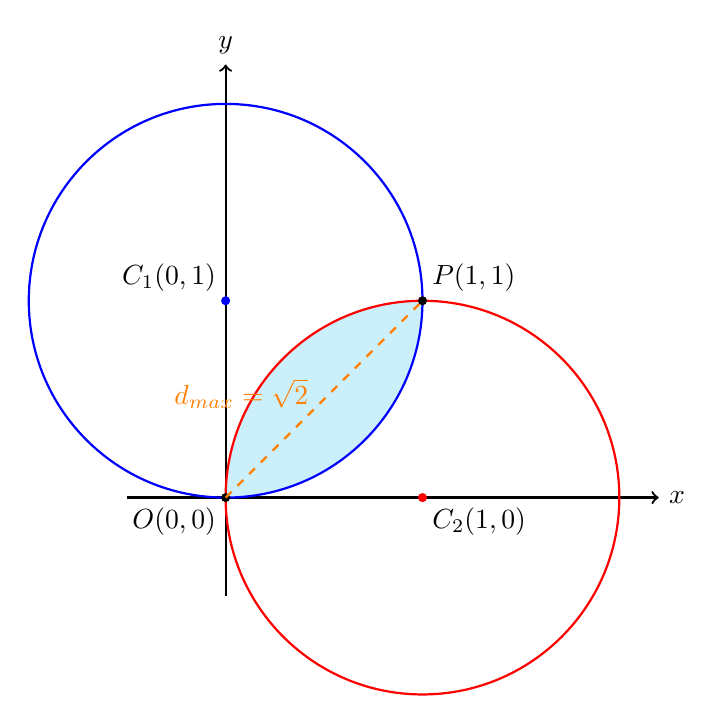
\begin{tikzpicture}[scale=2.5] % 放大比例以提升清晰度
    % 绘制坐标轴
    \draw[->, thick] (-0.5, 0) -- (2.2, 0) node[right] {$x$};
    \draw[->, thick] (0, -0.5) -- (0, 2.2) node[above] {$y$};

    % 填充两个圆的交集（可行域）
    \begin{scope}
        \clip (0,1) circle (1);
        \fill[cyan!20] (1,0) circle (1);
    \end{scope}

    % 绘制第一盏聚光灯的圆 C1(0, 1)
    \draw[blue, thick] (0,1) circle (1);
    \filldraw[blue] (0,1) circle (0.02) node[above left, text=black] {$C_1(0,1)$};

    % 绘制第二盏聚光灯的圆 C2(1, 0)
    \draw[red, thick] (1,0) circle (1);
    \filldraw[red] (1,0) circle (0.02) node[below right, text=black] {$C_2(1,0)$};

    % 标记原点 O(0,0) - 舞台中心
    \filldraw[black] (0,0) circle (0.02) node[below left] {$O(0,0)$};

    % 标记最远点 P(1,1)
    \filldraw[black] (1,1) circle (0.02) node[above right] {$P(1,1)$};

    % 绘制原点到最远点的距离线段（橘色虚线）
    \draw[dashed, thick, orange] (0,0) -- (1,1) node[midway, left, xshift=-2pt, yshift=2pt] {$d_{max} = \sqrt{2}$};

\end{tikzpicture}
\end{figure}

上面的图展示了第 1 组测试数据中的聚光灯光照区，可以发现 A 能走到的最远点为 $(1, 1)$, 答案即为 $d = \sqrt{2}$.

第 2 组测试数据的光照区除了原点外没有别的相交区域了，因此 A 能走到的最远点即为原点 $(0, 0)$，答案为 $0$.

% \subsection{提示}


\newpage
\section[B. 回响形态]{\myboxii{      \BF{\TT{B}}} 回响形态}

\textit{运行时间限制}   1 second

\textit{内存使用限制} 1 Gigabyte

\textit{读入文件} \qquad 标准输入

\textit{输出文件} \qquad 标准输出


\begin{quote}
	\textit{你构造序列成功了？}

	\textit{你构造序列成功}
\end{quote}

\subsection{题目描述}

构造王国还在追击小 T...

定义一个长度为 $n$ 的序列的前缀 $\max$ 序列 $x$ 为 $x_i = \max\{a_j : 1 \le j \le i\}$, 前缀 $\min$ 序列 $y$ 为 $y_i = \min\{a_j : 1 \le j \le i\}$.

对于给定的 $n$ 和 $k$, 请构造\BF{两个}满足如下条件的长度为 $n$ 的序列 $a$ 和 $b$, 如果不存在满足下述条件的两个序列，请报告无解：

\begin{itemize}
	\item $a$ 和 $b$ 为 $1$ 到 $n$ 的排列。
	\item $a$ 和 $b$ 有至少一项不同，也即存在 $i$ 满足 $a_i \ne b_i$.
	\item 对于 $a$ 和 $b$ 的中的任意一个序列，记其前缀 $\max$ 序列为 $x$, 前缀 $\min$ 序列为 $y$, 需要满足:
	\[
		\sum_{i=1}^n (x_i - y_i) = k.
	\]
\end{itemize}

\subsection{输入格式}

第一行输入一个整数 $T$ ($1 \le T \le 10^5$), 表示测试数据的数量。

每组测试数据一行输入两个整数 $n$ 和 $k$ ($2 \le n \le 10^5, 0 \le k \le 10^{10}$), 表示序列的长度和前缀 $\max$ 和 $\min$ 的差。

保证所有测试数据的 $\sum n \le 3 \times 10^5$.

\subsection{输出格式}

对于每组测试数据，若存在满足条件的两个序列则输出两行。

第一行输出 $n$ 个整数 $a_1$, $a_2$, $\ldots$, $a_n$ 表示你构造的第一个序列 $a$.

随后一行输出 $n$ 个整数 $b_1$, $b_2$, $\ldots$, $b_n$ 表示你构造的第二个序列 $b$.

若不存在满足条件的两个序列，则输出一行一个整数 $-1$.

如果有多个合法的答案则你可以输出其中任意一个。

\subsection{样例 1}

\begin{minipage}{\linewidth}
	\begin{minipage}[t]{0.49\linewidth}
		\begin{lstlisting}[title=\texttt{standard input}]
3
2 1
2 0
5 12
\end{lstlisting}
	\end{minipage}
	\begin{minipage}[t]{0.49\linewidth}
		\begin{lstlisting}[title=\texttt{standard output}]
1 2
2 1
-1
1 3 4 2 5 
1 2 4 5 3 
\end{lstlisting}
	\end{minipage}
\end{minipage}


\subsection{样例 1 解释}

对于第 3 组测试数据，我们验证第二个序列也就是 $b$ 序列是否符合条件：

\begin{itemize}
	\item $\{1, 2, 4, 5, 3\}$ 是一个 $1$ 到 $5$ 的排列，因为其中各个整数都出现且仅出现了一次。
	\item 第二项 $a_2 = 3$, $b_2 = 2$, $a_2 \ne b_2$.
	\item 其前缀 $\max$ 序列为 $x = \{1, 2, 4, 5, 5\}$, 前缀 $\min$ 序列为 $y = \{1, 1, 1, 1, 1\}$, 即得
	\[
		\sum_{i=1}^n (x_i - y_i) = (1 - 1) + (2 - 1) + (4 - 1) + (5 - 1) + (5 - 1) = 0 + 1 + 3 + 4 + 4 = 12 = k.
	\]
\end{itemize}

\subsection{提示}

一个 $1$ 到 $n$ 的排列是一个长度为 $n$ 且其中每个 $1$ 到 $n$ 的整数都出现且仅出现一次的序列。


\newpage
\section[C. 星之所在]{\myboxiii{      \BF{\TT{C}}} 星之所在}

\textit{运行时间限制}   1 second

\textit{内存使用限制} 1 Gigabyte

\textit{读入文件} \qquad 标准输入

\textit{输出文件} \qquad 标准输出


\begin{quote}
	\textit{Star farming 是我国古代的伟大发现。}
\end{quote}

\subsection{题目描述}

Ph\textbf{eo}nix 来到了外太空，这里有 $n$ 个星系，它们的编号分别为 $1$, $2$, $\ldots$, $n$, 这些星系通过 $n - 1$ 条双向虫洞通道相互连接，每个星系都可以经由这些虫洞通道相互抵达。

每个星系包含一些恒星，$i$ 号星系拥有的恒星数量为 $s_i$.

Pheonix 将要进行 $q$ 次星系之间穿越虫洞的旅行，在一次旅行中 Pheonix 不会重复前往去过的星系。


Pheonix 对天文了解有限，但 Pheonix 的数学观察力很敏锐，对于每次旅行他想要询问小 T 这样的问题：

\begin{itemize}
	\item 将从星系 $x$ 到星系 $y$ 的虫洞旅行中会经过的星系（包括起点和终点）的恒星数量放进一个可重集合 $S$ 中，也即 $S = \{s_i : i\ \text{在} \ x \ \text{到}\  y\ \text{的路径上}\}$.
	\item $S$ 中是否存在元素满足其出现次数严格大于 $\frac{|S|}{k}$? 其中 $k$ 是 Pheonix 在每次提问中指定的一个整数。若有则求出有哪些。
\end{itemize}

请帮助小 T 回答这些问题。

\subsection{输入格式}

第一行输入一个整数 $T$ ($ 1 \le T \le 10^5$), 表示测试数据的数量。

每组测试数据第一行输入两个整数 $n$ 和 $q$ ($2 \le n \le 10^5, 1 \le q \le 10^5$), 表示星系数量和 Pheonix 的旅行次数。

随后一行输入 $n$ 个整数 $s_1$, $s_2$, $\ldots$, $s_n$ ($1 \le s_i \le n$), 分别表示这些星系所拥有的恒星数量。

随后 $n - 1$ 行每行输入两个整数 $u$ 和 $v$ ($1 \le u, v \le n, u \ne v$), 表示存在一条连接 $u$ 和 $v$ 的虫洞通道。

随后 $q$ 行每行输入 $3$ 个整数 $x$, $y$, $k$ ($1 \le x, y \le n, 2 \le k \le n, x \ne y$), 表示 Pheonix 的一次旅行的起点和终点，以及提问的参数。

保证所有测试数据的 $\sum n, \sum q, \sum k \le 3 \times 10^5$, 保证每组测试数据中的虫洞通道满足每个星系都可以经由这些虫洞通道相互抵达。

\subsection{输出格式}

对于每组测试数据输出 $q$ 行，第 $i$ 行输出第 $i$ 次提问的答案：
\begin{itemize}
	\item 若存在 $S$ 中元素满足其出现次数严格大于 $\frac{|S|}{k}$, 则按照恒星数量大小从小到大输出（而非按照出现次数）恒星数量。
	\item 否则输出一个整数 $-1$.
\end{itemize}

\subsection{样例 1}

\begin{minipage}{\linewidth}
	\begin{minipage}[t]{0.49\linewidth}
		\begin{lstlisting}[title=\texttt{standard input}]
2
6 4
1 2 2 1 2 3
1 2
2 3
2 4
4 5
5 6
3 6 2
1 4 3
1 6 2
1 5 3
7 5
1 2 1 3 2 2 4
1 2
1 3
2 4
2 5
3 6
6 7
4 5 2
4 7 3
5 6 4
3 1 2
7 5 2
\end{lstlisting}
	\end{minipage}
	\begin{minipage}[t]{0.49\linewidth}
		\begin{lstlisting}[title=\texttt{standard output}]
2
1
-1
1 2
2
-1
1 2
1
-1
\end{lstlisting}
	\end{minipage}
\end{minipage}


\subsection{样例 1 解释}


\begin{figure}[htbp]
   \centering
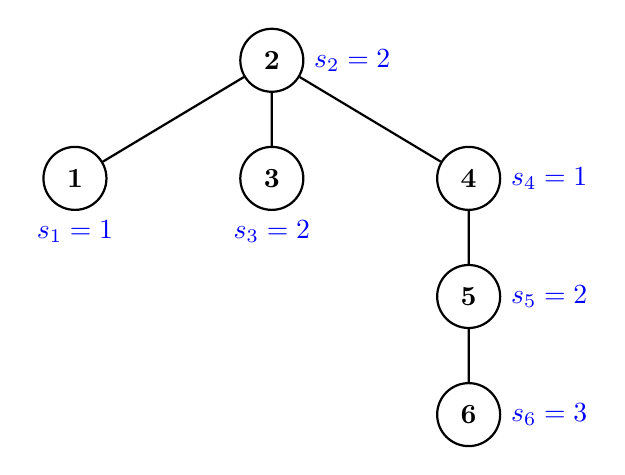
\begin{tikzpicture}[
    level 1/.style={sibling distance=2.5cm},
    level 2/.style={sibling distance=2cm},
    level distance=1.5cm,
    galaxy/.style={circle, draw=black, thick, minimum size=0.8cm, font=\bfseries},
    edge from parent/.style={draw=black, thick}
]

% 根节点：星系 2
\node[galaxy, label={[text=blue]right:$s_2=2$}] {2}
    % 星系 2 的三个子节点：1, 3, 4
    child { node[galaxy, label={[text=blue]below:$s_1=1$}] {1} }
    child { node[galaxy, label={[text=blue]below:$s_3=2$}] {3} }
    child { node[galaxy, label={[text=blue]right:$s_4=1$}] {4}
        % 星系 4 的子节点：5
        child { node[galaxy, label={[text=blue]right:$s_5=2$}] {5}
            % 星系 5 的子节点：6
            child { node[galaxy, label={[text=blue]right:$s_6=3$}] {6} }
        }
    };

\end{tikzpicture}
\end{figure}

上面的图展示了第 1 组测试数据的虫洞链接情况和恒星数量。

第 1 组询问从 $3$ 号星系到 $6$ 号星系，参数为 $2$, 经过的星系编号为 $3 \rightarrow 2 \rightarrow 4 \rightarrow 5 \rightarrow 6$, 恒星数量分别为 $S = \{2, 2, 1, 2, 3\}$, 满足出现次数严格大于阈值 $\frac{|S|}{k} = 2.5$ 的恒星数量为 $2$.






\newpage
\section[D. 左灯右行]{\myboxiv{      \BF{\TT{D}}} 左灯右行}

\textit{运行时间限制}   1 second

\textit{内存使用限制} 1 Gigabyte

\textit{读入文件} \qquad 标准输入

\textit{输出文件} \qquad 标准输出


\begin{quote}
	\textit{我爱你有种}
\end{quote}

\BF{本题和试题 \myboxv{\BF{\TT{E}}} 右灯左行共用相同的背景，两道题之间有较大的关系，建议在尝试其中一题前首先阅读另一题的文本。}

\BF{这是一道交互题。}

\subsection{题目描述}

小 T 面对 T 城的地铁图犯了难 ...

具体而言，这座城市在 E 河两岸，北岸有 $n$ 个地铁站点 $N_1$, $N_2$, $\ldots$, $N_n$, 南岸有 $n$ 个地铁站点 $S_1$, $S_2$, $\ldots$, $S_n$.

T 城总共有 $n - 1$ 条地铁线路，每条线路都是环线，其中第 $i$ 条环线连接的地铁站是 $N_i - N_{i + 1} - S_{i + 1} - S_i - N_i$, 但这些地铁环线都是单向运行的，可能是 $N_i \leftarrow N_{i + 1} \leftarrow S_{i + 1} \leftarrow S_i \leftarrow N_i$ 也可能是 $N_i \rightarrow N_{i + 1} \rightarrow S_{i + 1} \rightarrow S_i \rightarrow N_i$.


每条环线都有一个价目表 $u_i$, $d_i$, $l_i$, $r_i$, 分别表示这 4 个相邻站 ($N_i - N_{i + 1}$, $S_i - S_{i + 1}$, $N_i - S_i$ 和 $N_{i + 1} - S_{i + 1}$) 之间坐一站地铁移动的价格，注意坐一站地铁的方向由地铁的运行方向而定，可能是 $N_i \rightarrow N_{i + 1}$ 也可能是 $N_{i} \leftarrow N_{i + 1}$.

遗憾的是，时空黑洞吞噬了价目表上这些环线的运行方向和价格，小 T 准备求助大 K 的帮助来得知这些地铁的运行方向。

大 K 知道地铁的运行方向，不过，小 T 可以为每条环线的四段相邻站边重新任意指定一组价格；大 K 知道真实的运行方向，并会根据这些指定价格回答小 T 的询问。

小 T 可以询问他至多 $3\,500$ 个问题：

\begin{itemize}
	\item 地铁站 $x$(可以是 $N_i$ 也可以是 $S_i$, 下略) 到地铁站 $y$ 坐地铁，在小 T 指定的地铁价目表下，至少需要支付多少地铁费用？
   \item 若不同环线连接同一对相邻站，则这些边同时存在并且都可以使用。一次旅行的费用为所经过边权之和，站点间换乘不额外收费。
\end{itemize}


在询问完这些问题后，小 T 需要和大 K 确认每条地铁的运行方向。

请帮助小 T 解决这个问题。

请注意，地铁线路的方向是预先确定的，它们不会在交互的过程中更改，换言之交互器\BF{不是}自适应的。

\subsection{交互协议}

本题每个测试点只有一组测试数据。

第一行输入一个整数 $n$ ($2 \le n \le 10^5$), 表示参数，其中地铁站共 $2n$ 座，环线共 $n - 1$ 条。

你首先需要输出 $n - 1$ 行，其中第 $i$ 行输出 $4$ 个整数 $u_i$, $d_i$, $l_i$, $r_i$, 分别表示第 $i$ 条环线上 $N_i - N_{i + 1}$, $S_i - S_{i + 1}$, $N_i - S_i$ 和 $N_{i + 1} - S_{i + 1}$ 这四个相邻站之间的移动价格，你需要保证这四个整数在 $[0, 10^9]$ 之间。

随后你将会直接开始交互，每一次交互你可以以下面的格式向交互器询问问题：

\begin{itemize}
   \item 输出一行，首先输出一个字符 \TT{?} 表示你询问一次，随后输出 $4$ 个元素 $S_x$, $id_x$, $S_y$, $id_y$, 其中你需要保证 $S_x, S_y \in \{\mathtt{N}, \mathtt{S}\}$, $id_x, id_y \in \{m \in \mathbb{N} : 1 \le m \le n\}$, 表示小 T 需要询问大 K 位于 $S_x$ 岸的第 $id_x$ 个地铁站 $(S_x)_{id_x}$ 到位于 $S_y$ 岸的第 $id_y$ 个地铁站 $(S_y)_{id_y}$ 之间至少需要支付多少地铁费用。
   \item 若你的输入合法并且没有超出询问限制，交互器会给出一行一个整数 $d$ 供输入表示这两个站点之间最少需要的地铁费用。
   \item 若你询问的问题超出了对应的询问次数限制，交互器会输出一个整数 $-1$ 并结束你的交互进程，此时你会获得\textit{答案错误}的评测结果。
\end{itemize}

若你已经得到地铁方向的话，请按照以下的格式输出答案：

\begin{itemize}
   \item 输出一行，首先输出一个字符 \TT{!}, 随后输出一个长度为 $n - 1$ 的字符串 $S$, 其中第 $i$ 个字符 $S_i \in \{\mathtt{I}, \mathtt{O}\}$, 若 $S_i = \mathtt{I}$ 则表示第 $i$ 条环线的方向为 $N_i \leftarrow N_{i + 1} \leftarrow S_{i + 1} \leftarrow S_i \leftarrow N_i$, 若 $S_i = \mathtt{O}$ 则表示第 $i$ 条环线的方向为 $N_i \rightarrow N_{i + 1} \rightarrow S_{i + 1} \rightarrow S_i \rightarrow N_i$.
\end{itemize}

在完成输出答案后，你应当安全退出。

每次输出都需要输出换行并且刷新缓冲区，否则你可能会得到意料之外的结果。

为了刷新缓冲区，你可以：

\begin{itemize}
   \item 对于 C 或者 C++, 使用 \TT{fflush(stdout)} 或 \TT{cout.flush()}。
   \item 对于 Java 或 Kotlin, 使用 \TT{System.out.flush()}。
   \item 对于 Python, 使用 \TT{stdout.flush()}。
\end{itemize}

\subsection{样例 1}

\begin{minipage}{\linewidth}
	\begin{minipage}[t]{0.49\linewidth}
		\begin{lstlisting}[title=\texttt{standard input}]
3
10
12
\end{lstlisting}
	\end{minipage}
	\begin{minipage}[t]{0.49\linewidth}
		\begin{lstlisting}[title=\texttt{standard output}]
10 3 1 2
10 10 1 1
? N 1 N 2
? N 2 N 3
! OI
\end{lstlisting}
	\end{minipage}
\end{minipage}


\subsection{样例 1 解释}

\begin{figure}[htbp]
   \centering
\begin{tikzpicture}[
  >=Stealth,
  station/.style={circle,draw,thick,minimum size=10mm,font=\large},
  bank/.style={thick},
  solid/.style={thick,->},
  rdashed/.style={thick,dashed,->},
  edgecost/.style={font=\Large, inner sep=0pt}
]

% --- coordinates / stations ---
\node[station] (N1) at (0, 2.2) {$N_1$};
\node[station] (N2) at (4, 2.2) {$N_2$};
\node[station] (N3) at (8, 2.2) {$N_3$};

\node[station] (S1) at (0,-2.2) {$S_1$};
\node[station] (S2) at (4,-2.2) {$S_2$};
\node[station] (S3) at (8,-2.2) {$S_3$};

% --- banks (text NOT on the line) ---
\draw[bank] (-1.5, 0.9) -- (9.5, 0.9);
\node[font=\Large] at (9.4, 1.25) {North bank};

\draw[bank] (-1.5,-0.9) -- (9.5,-0.9);
\node[font=\Large] at (9.4,-0.55) {South bank};

% --- Ring 1 = O : N1->N2->S2->S1->N1 ---
\draw[solid] (N1) -- (N2) node[midway,above=8pt,edgecost] {10};
\draw[solid] (N2) -- (S2) node[midway,left=10pt,edgecost] {2};


\draw[solid] (S2) -- (S1) node[midway,below=8pt,edgecost] {3};
\draw[solid] (S1) -- (N1) node[midway,left=10pt,edgecost] {1};

% --- Ring 2 = I : N3->N2, S3->N3, S2->S3, N2->S2 ---
\draw[rdashed] (N3) -- (N2) node[midway,above=8pt,edgecost] {10};
\draw[rdashed] (S3) -- (N3) node[midway,right=10pt,edgecost] {2};
\draw[rdashed] (S2) -- (S3) node[midway,below=8pt,edgecost] {10};

% --- the requested "double edge" on N2->S2: one solid + one dashed ---
% dashed copy slightly shifted to the right, so both are visible
\draw[rdashed] ([xshift=3pt]N2.south) -- ([xshift=3pt]S2.north)
  node[midway,right=14pt,edgecost] {1};

% --- ring labels ---
\node[font=\Large] at (2.0, 0) {Ring 1};
\node[font=\Large] at (6.0, 0) {Ring 2};

\end{tikzpicture}


\end{figure}
上面的图展示了地铁的运行方向和小 T 的价格标注。

请注意样例中的交互过程仅供参考，实际交互过程并不唯一，且这一示例的交互过程不一定是可行的或是最优的，本题的样例不会在附加文件中出现。






\newpage
\section[E. 右灯左行]{\myboxv{      \BF{\TT{E}}} 右灯左行}

\textit{运行时间限制}   1 second

\textit{内存使用限制} 1 Gigabyte

\textit{读入文件} \qquad 标准输入

\textit{输出文件} \qquad 标准输出


\begin{quote}
	\textit{的冲突，}
\end{quote}

\BF{本题和试题 \myboxiv{\BF{\TT{D}}} 左灯右行共用相同的背景，两道题之间有较大的关系，建议在尝试其中一题前首先阅读另一题的文本。}

\BF{这不是一道交互题。}

\subsection{题目描述}

小 T 面对 T 城的地铁图犯了难 ...

具体而言，这座城市在 E 河两岸，北岸有 $n$ 个地铁站点 $N_1$, $N_2$, $\ldots$, $N_n$, 南岸有 $n$ 个地铁站点 $S_1$, $S_2$, $\ldots$, $S_n$.

T 城总共有 $n - 1$ 条地铁线路，每条线路都是环线，其中第 $i$ 条环线连接的地铁站是 $N_i - N_{i + 1} - S_{i + 1} - S_i - N_i$, 但这些地铁环线都是单向运行的，可能是 $N_i \leftarrow N_{i + 1} \leftarrow S_{i + 1} \leftarrow S_i \leftarrow N_i$ 也可能是 $N_i \rightarrow N_{i + 1} \rightarrow S_{i + 1} \rightarrow S_i \rightarrow N_i$.


每条环线都有一个价目表 $u_i$, $d_i$, $l_i$, $r_i$, 分别表示这 4 个相邻站 ($N_i - N_{i + 1}$, $S_i - S_{i + 1}$, $N_i - S_i$ 和 $N_{i + 1} - S_{i + 1}$) 之间坐一站地铁移动的价格，注意坐一站地铁的方向由地铁的运行方向而定，可能是 $N_i \rightarrow N_{i + 1}$ 也可能是 $N_{i} \leftarrow N_{i + 1}$.

高兴的是，时空白洞吐出了价目表上这些环线的运行方向和价格，大 K 准备求助小 T 来得到一些通过地铁移动的价格。

大 K 会告诉小 T 这些环线的运行方向和价目表，随后小 T 需要回答 $q$ 个问题：

\begin{itemize}
  \item  地铁站 $x$(可以是 $N_i$ 也可以是 $S_i$, 下略) 到地铁站 $y$ 坐地铁，在给定的地铁价目表下，至少需要支付多少地铁费用？
  \item 若不同环线连接同一对相邻站，则这些边同时存在并且都可以使用。一次旅行的费用为所经过边权之和，站点间换乘不额外收费。
\end{itemize}

请帮助小 T 解决这个问题。

\subsection{输入格式}

第一行输入一个整数 $T$ ($ 1 \le T \le 10^5$), 表示测试数据的数量。

每组测试数据第一行输入两个整数 $n$ 和 $q$ ($2 \le n \le 10^5, 1 \le q \le 10^5$), 表示参数和询问数量，其中地铁站共 $2n$ 座，环线共 $n - 1$ 条。

随后输入 $n - 1$ 行，其中第 $i$ 行输入 $4$ 个整数 $u_i$, $d_i$, $l_i$, $r_i$($0 \le u_i, d_i, l_i, r_i \le 10^9$), 分别表示第 $i$ 条环线上 $N_i - N_{i + 1}$, $S_i - S_{i + 1}$, $N_i - S_i$ 和 $N_{i + 1} - S_{i + 1}$ 这四个相邻站之间的移动价格。

随后输入一行一个长度为 $n - 1$ 的字符串 $S$, 其中第 $i$ 个字符 $S_i \in \{\mathtt{I}, \mathtt{O}\}$, 若 $S_i = \mathtt{I}$ 则表示第 $i$ 条环线的方向为 $N_i \leftarrow N_{i + 1} \leftarrow S_{i + 1} \leftarrow S_i \leftarrow N_i$, 若 $S_i = \mathtt{O}$ 则表示第 $i$ 条环线的方向为 $N_i \rightarrow N_{i + 1} \rightarrow S_{i + 1} \rightarrow S_i \rightarrow N_i$.

随后输入 $q$ 行每行输入 $4$ 个元素 $S_x$, $id_x$, $S_y$, $id_y$, ($S_x, S_y \in \{\mathtt{N}, \mathtt{S}\}$, $id_x, id_y \in \{m \in \mathbb{N} : 1 \le m \le n\}$), 表示大 K 询问小 T 位于 $S_x$ 岸的第 $id_x$ 个地铁站 $(S_x)_{id_x}$ 到位于 $S_y$ 岸的第 $id_y$ 个地铁站 $(S_y)_{id_y}$ 之间至少需要支付多少地铁费用。

保证所有测试数据输入中的 $\sum n \le 3 \times 10^5$, $\sum q \le 3 \times 10^5$.

\subsection{输出格式}

每组测试数据输出 $q$ 行，第 $i$ 行输出一个整数 $d$ 表示小 T 收到的第 $i$ 个询问的答案，也即 $(S_x)_{id_x}$ 到 $(S_y)_{id_y}$ 至少需要支付多少地铁费用。


\subsection{样例 1}

\begin{minipage}{\linewidth}
	\begin{minipage}[t]{0.49\linewidth}
		\begin{lstlisting}[title=\texttt{standard input}]
3
3 5
10 3 1 2
10 10 1 1
OI
N 1 N 2
N 2 N 3
N 2 S 2
S 2 N 2
N 1 N 1
6 1
5 1 7 3
2 6 3 4
6 8 1 7
10 0 7 8
4 5 4 9
IOIOI
N 4 S 4
6 1
4 5 7 6
5 0 9 1
1 5 1 5
10 4 7 1
2 1 3 3
OIOIO
S 6 S 4
\end{lstlisting}
	\end{minipage}
	\begin{minipage}[t]{0.49\linewidth}
		\begin{lstlisting}[title=\texttt{standard output}]
10
12
1
14
0
14
17
\end{lstlisting}
	\end{minipage}
\end{minipage}


\subsection{样例 1 解释}

\begin{figure}[htbp]
   \centering
\begin{tikzpicture}[
  >=Stealth,
  station/.style={circle,draw,thick,minimum size=10mm,font=\large},
  bank/.style={thick},
  solid/.style={thick,->},
  rdashed/.style={thick,dashed,->},
  edgecost/.style={font=\Large, inner sep=0pt}
]

% --- coordinates / stations ---
\node[station] (N1) at (0, 2.2) {$N_1$};
\node[station] (N2) at (4, 2.2) {$N_2$};
\node[station] (N3) at (8, 2.2) {$N_3$};

\node[station] (S1) at (0,-2.2) {$S_1$};
\node[station] (S2) at (4,-2.2) {$S_2$};
\node[station] (S3) at (8,-2.2) {$S_3$};

% --- banks (text NOT on the line) ---
\draw[bank] (-1.5, 0.9) -- (9.5, 0.9);
\node[font=\Large] at (9.4, 1.25) {North bank};

\draw[bank] (-1.5,-0.9) -- (9.5,-0.9);
\node[font=\Large] at (9.4,-0.55) {South bank};

% --- Ring 1 = O : N1->N2->S2->S1->N1 ---
\draw[solid] (N1) -- (N2) node[midway,above=8pt,edgecost] {10};
\draw[solid] (N2) -- (S2) node[midway,left=10pt,edgecost] {2};


\draw[solid] (S2) -- (S1) node[midway,below=8pt,edgecost] {3};
\draw[solid] (S1) -- (N1) node[midway,left=10pt,edgecost] {1};

% --- Ring 2 = I : N3->N2, S3->N3, S2->S3, N2->S2 ---
\draw[rdashed] (N3) -- (N2) node[midway,above=8pt,edgecost] {10};
\draw[rdashed] (S3) -- (N3) node[midway,right=10pt,edgecost] {1};
\draw[rdashed] (S2) -- (S3) node[midway,below=8pt,edgecost] {10};

% --- the requested "double edge" on N2->S2: one solid + one dashed ---
% dashed copy slightly shifted to the right, so both are visible
\draw[rdashed] ([xshift=3pt]N2.south) -- ([xshift=3pt]S2.north)
  node[midway,right=14pt,edgecost] {1};

% --- ring labels ---
\node[font=\Large] at (2.0, 0) {Ring 1};
\node[font=\Large] at (6.0, 0) {Ring 2};

\end{tikzpicture}
\end{figure}

上面的图展示了第 1 组测试数据中地铁的运行方向和价目表。







\newpage
\section[F. 迷路日]{\myboxvi{      \BF{\TT{F}}} 迷路日}

\textit{运行时间限制}   1 second

\textit{内存使用限制} 1 Gigabyte

\textit{读入文件} \qquad 标准输入

\textit{输出文件} \qquad 标准输出

\begin{quote}
   \textit{月が話しかけてきた\\
そして不思議な力をくれた\\}
   \textit{也许该交换一下标题。}
\end{quote}

\subsection{题目描述}

小 T 来到了 T 城，她要前往一个 Livehouse 演出。

T 城可以用一个无限大的欧氏二维平面表示，$y$ 轴正方向表示正北 (N) 方向，$x$ 轴正方向表示正东 (E) 方向，$y$ 轴负方向表示正南 (S) 方向，$x$ 轴负方向表示正西 (W) 方向。

小 T 初始站在 $(x_{t}, y_{t})$ 的位置，初始面向正东、正南、正西、正北四个方向中的一个，她要去的 Livehouse 位于 $(x_l, y_l)$.

她每次移动可以选择下面两种中的一个：

\begin{itemize}
   \item 直行，沿当前方向走一个单位长度。
   \item 右转，将小 T 面对的方向顺时针转 $90^\circ$ （北转向东，东转向南，南转向西，西转向北）。
\end{itemize}

注意小 T 不能左转或掉头。

请求出在上述条件下，小 T 至少要\textbf{右转}几次才能到 Livehouse, 可以证明在这些规则下总能到达目标位置。

\subsection{输入格式}

第一行输入一个整数 $T$ ($1 \le T \le 10^5$), 表示测试数据的数量。

每组测试数据一行输入 5 个元素 $x_t$, $y_t$, $dir$, $x_l$, $y_l$($x_t, y_t, x_l, y_l \in \{n \in \mathbb{Z} : -10^9 \le n \le 10^9$ \}, $dir \in \{\text{N}, \text{E}, \text{S}, \text{W}\}$), 分别表示小 T 所在的位置，小 T 初始面对的方向，Livehouse 的位置。

\subsection{输出格式}

对于每组测试数据，输出一行一个整数，表示在上述条件下，小 T 至少要\textbf{右转}几次才能到 Livehouse.

\subsection{样例 1}

\begin{minipage}{\linewidth}
   \begin{minipage}[t]{0.49\linewidth}
      \begin{lstlisting}[title=\texttt{standard input}]
8
0 0 E 3 -2
1 1 N 0 1
10 10 E 10 10
-9 2 E 3 2
0 -7 E -1 -4
0 6 E -4 6
10 -9 S 10 9
1 -3 N -1 0
\end{lstlisting}
   \end{minipage}
   \begin{minipage}[t]{0.49\linewidth}
      \begin{lstlisting}[title=\texttt{standard output}]
1
3
0
0
3
2
2
3
\end{lstlisting}
   \end{minipage}
\end{minipage}

\subsection{样例 1 解释}

对于第 $1$ 组测试数据，首先向东走 $3$ 步到达 $(3,0)$, 随后右转朝向南，再向南走 $2$ 步到 $(3, -2)$.

对于第 $2$ 组测试数据，首先右转三次朝向西，随后走 $1$ 步到达 $(0, 1)$.

对于第 $3$ 组测试数据，起点和终点重合因此不需要右转。
\newpage
\section[G. 朝复习]{\myboxvii{      \BF{\TT{G}}} 朝复习}

\textit{运行时间限制}   1 second

\textit{内存使用限制} 1 Gigabyte

\textit{读入文件} \qquad 标准输入

\textit{输出文件} \qquad 标准输出


\begin{quote}
	\textit{计算机科学：复习 (Computer Science: Go Over, known as \_\_\_ ) 是一个在全球流行的事项。}
\end{quote}

\BF{本题和试题 \myboxviii{\BF{\TT{H}}} 朝复夕没有关系。}

\subsection{题目描述}

TSUCE(Time-Space Union of Coding Experts) 准备举办 TSUCE Programming Duel Cup，这是两个选手之间的算法竞赛单挑赛！

赛制如下，请留意其中 $n$ 和 $m$ 的含义：
\begin{itemize}
	\item 每场比赛由两名选手对战，一场比赛有且仅有一名获得胜利的选手，没有平局。
	\item 一场由一节常规时间比赛 + 若干节加时赛组成（可能只有 $0$ 节加时赛），常规时间包含 $2n$ 轮比赛，一节加时赛包含 $2m$ 轮比赛，一轮比赛有且仅有一名胜者。
	\item 常规时间内获得 $n + 1$ 轮胜利的选手将获得整场比赛的胜利，比赛将立刻结束。
	\item 常规时间 $2n$ 轮后若未分胜负（比分 $n:n$）后会进入加时赛，单节加时内获得 $m + 1$ 轮胜利的选手将获得整场比赛的胜利，比赛将立刻结束。
	\item 一节加时赛后仍然未分胜负则将进入下一节加时，直到决出胜负。
	\item 最后的比分为双方在整场比赛中各自赢得的轮数。
\end{itemize}

遗憾的是，记分员小 T 的数据库坏掉了，他只记得全部 $k$ 场比赛的比分，但他不记得和赛制相关的 $n$ 和 $m$ 了。

请帮助他确定是否存在一组合法的正整数 $n$ 和 $m$ 使得这些比分都是在该赛制下合法的比分。

\subsection{输入格式}

第一行输入一个整数 $T$ ($1 \le T \le 10^5$), 表示测试数据的数量。

每组测试数据第一行输入一个整数 $k$ ($1 \le k \le 10^5$), 表示记录的比赛场数。

随后 $k$ 行输入两个整数 $a$ 和 $b$ ($0 \le a, b \le 10^{18}, |a - b| \ge 2$), 表示小 T 数据库中记录的一场比赛的比分。

保证所有测试数据输入中的 $\sum k \le 3 \times 10^5$.

\subsection{输出格式}

对于每组测试数据，如果存在一个合法的 $n$ 和 $m$ 使得这些比分都是在该赛制下合法的比分，则输出一行一个字符串 \texttt{YES}, 否则输出一行一个字符串 \texttt{NO}.

注意评测时不会区分 \TT{YES} 和 \TT{NO} 的大小写，换言之当答案是肯定的时候输出 \TT{yes}, \TT{YES}, \TT{Yes}, \TT{YeS} 等都会被认为是正确的。

\subsection{样例 1}

\begin{minipage}{\linewidth}
	\begin{minipage}[t]{0.49\linewidth}
		\begin{lstlisting}[title=\texttt{standard input}]
6
3
16 14
10 16
19 22
2
11 16
19 22
5
2 13
16 12
9 13
13 10
20 22
2
5 7
5 9
3
0 5
5 2
11 7
2
6 9
9 6
\end{lstlisting}
	\end{minipage}
	\begin{minipage}[t]{0.49\linewidth}
		\begin{lstlisting}[title=\texttt{standard output}]
YES
YES
YES
NO
YES
YES
\end{lstlisting}
	\end{minipage}
\end{minipage}


\subsection{样例 1 解释}

对于第 $3$ 组测试数据，可以发现 $n = 12$, $m = 3$ 是一个合理的解，这样子比赛会经过如上的过程：

\begin{itemize}
	\item 第一场 $2:13$, 常规时间 B 选手率先拿下 $n + 1 = 13$ 局胜利以结束比赛。
	\item 第二场 $16:12$, 常规时间 $12:12$ 战平，第一节加时 A 选手 $4:0$ 直落对手，拿下了 $m + 1 = 4$ 局胜利。
	\item 第三场第四场比赛分别以 $9:13$ 和 $13:10$ 在常规时间内结束。
	\item 第五场比赛常规时间战成 $12:12$, 第一节加时和第二节加时双方都以 $3:3$ 战平，比赛以 $18:18$ 进入第三节加时，最终 B 选手在第三节加时 $4:2$ 战胜对手，最终比分 A $20:22$ B.
\end{itemize}






\newpage
% \section[H. 剪切线]{\myboxviii{      \BF{\TT{H}}} 剪切线}

\textit{运行时间限制}   1 second

\textit{内存使用限制} 1 Gigabyte

\textit{读入文件} \qquad 标准输入

\textit{输出文件} \qquad 标准输出

\begin{quote}
   \textit{【数据|【数据}

   \textit{删除】|删除】}
\end{quote}


\subsection{题目描述}

小 T 已经登神，他已经进入了高维的空间。

在一个 $d$ 维的高维长方体中，每一维的长度分别为 $n_1$, $n_2$, $\ldots$, $n_d$, 而这个长方体由 $\prod_{i=1}^{n} n_i = n_1n_2\ldots n_d$ 个小正方体组成, 每个小正方体的坐标分别为 $(a_1, a_2, \ldots, a_{d})$, 其中 $a_i$ 为整数且 $1 \le a_i \le n_i$.

小 T 选出了其中的 $m$ 个小正方体做了标记，其坐标分别为 $(c_{1, 1}, c_{1, 2}, \ldots, c_{1, d})$, $(c_{2, 1}, c_{2, 2}, \ldots, c_{2, d})$, $\ldots$, $(c_{m, 1}, c_{m, 2}, \ldots, c_{m, d})$, 同时每个被标记的小正方体都有一个分值 $p_1$, $p_2$, $\ldots$, $p_m$，同时他也生成了两个叫做 Alpha 和 Beta 的智能机器来做游戏。

从 Alpha 开始, Alpha 和 Beta 会依次轮流进行如下的操作，其中每次的操作都是给定的：

\begin{itemize}
   \item 当前回合的智能机器 $C$ 会选择一个维度 $D$,  记当前长方体在这个维数下的剩余长度为 $n_D'$, 智能机器同时会选择一个象征方向和层数的数 $k$, 保证 $0 < |k| < n_D'$,  将将高维长方体劈成两块并舍去其中的一块，具体如下：
   \begin{itemize}
      \item 若 $k > 0$, 则当前的长方体的第 $D$ 维的前 $|k|$ 层会被劈开并舍去；
      \item 若 $k < 0$, 则当前的长方体的第 $D$ 维的后 $|k|$ 层会被劈开并舍去；
   \end{itemize}
   \item 当前回合的智能机器 $C$ 劈开并舍去的小长方体中，其中每有一个被做标记的小正方体便得到其对应的分值。
\end{itemize}

上述的操作共进行了 $q$ 次, 请帮助小 T 计算出操作结束后 Alpha 和 Beta 所得的分数.

\subsection{输入格式}

第一行输入一个整数 $T$ ($1 \le T \le 10^5$), 表示数据组数。

每组数据第一行输入 3 个整数 $d$, $m$, $q$($1 \le d \le 10$, $1 \le m \le 2 \times 10^5$, $1 \le q \le 2 \times 10^5$), 分别表示长方体的维数，做了标记的小正方体的数量和智能机器所进行操作的次数。

接下来一行输入 $d$ 个整数 $d_1$, $d_2$, $\ldots$, $d_{n}$,($1 \le n_i \le 10^9$), 分别表示高维长方体每一维的长度。

接下来一行输入 $m$ 个整数 $p_1$, $p_2$, $\ldots$, $p_n$($1 \le p_i \le 10^9$), 分别表示每个小正方体的分值。

接下来 $m$ 行每行输入 $d$ 个整数 $c_{i, 1}$, $c_{i, 2}$, $\ldots$, $c_{i, d}$ 其中 $1 \le c_{i, j} \le n_j$, 表示这个被做了标记的小正方体的坐标。

接下来 $q$ 行每行输入两个整数 $D$ 和 $k$, 其中 $1 \le D \le d$, 分别表示当前回合的智能机器所选的维度和所选的象征方向和层数的数，具体含义如题意中所述。

保证每次操作都是合法的，即不会出现操作的维度长度不足的情况。

保证所有测试数据输入中的 $\sum (n \cdot d) \le 2 \times 10^6$, $\sum q \le  3 \times 10^5$.

\subsection{输出格式}

每组数据输出一行两个整数 $score_A$ 和 $score_B$, 分别操作结束后表示 Alpha 和 Beta 所得的分值。

\subsection{样例 1}
\begin{minipage}{\linewidth}
   \begin{minipage}[t]{0.49\linewidth}
      \begin{lstlisting}[title=\texttt{standard input}]
2
2 4 2
1 1 1 1
4 4
4 1
3 3
2 3
2 1
1 -2
2 1
1 3 3
12 34 56
100
20
50
90
1 -2
1 3
1 4
\end{lstlisting}
   \end{minipage}
   \begin{minipage}[t]{0.49\linewidth}
      \begin{lstlisting}[title=\texttt{standard output}]
2 1
0 0
\end{lstlisting}
   \end{minipage}
\end{minipage}


\subsection{样例 1 解释}

对于第 1 组样例，此时长方体是一个 $2$ 维的，令上下方向表示第 $1$ 维，左右方向表示第 $2$ 维，则其中被做了标记的小正方体用其对应的分数表示，如下所示：
\begin{table}[htbp]
      \begin{center}
         \begin{tabular}{|c|c|c|c|c|}
          \hline
          & 1 & 2 & 3 & 4 \\ \hline
          1 & .& .& .& . \\\hline
          2 & 1 & .& 1&. \\\hline
          3 &   .& .& 1 &.\\ \hline
          4 & 1 &. &. & .\\\hline
          % \hline
        \end{tabular}
      \end{center}
\end{table}


第一次操作由 Alpha 进行，操作后的长方体如下所示：

\begin{table}[htbp]
      \begin{center}
         \begin{tabular}{|c|c|c|c|c|}
          \hline
          & 1 & 2 & 3 & 4 \\ \hline
          1 & .& .& .& . \\\hline
          2 & 1 & .& 1&. \\\hline
          % \hline
        \end{tabular}
      \end{center}
\end{table}
\vspace{-2ex}
此时 Alpha 得 $2$ 分。

第二次操作由 Beta 进行，操作后的长方体如下所示：

\begin{table}[htbp]
      \begin{center}
         \begin{tabular}{|c|c|c|c|}
          \hline
          &  2 & 3 & 4 \\ \hline
          1 &  .& .& . \\\hline
          2 & .& 1&. \\\hline
          % \hline
        \end{tabular}
      \end{center}
\end{table}
\vspace{-2ex}
此时 Beta 得 $1$ 分，操作结束后 Alpha 和 Beta 所得的分数 分别为 $2$ 分和 $1$ 分。




% \newpage
\section[H. 朝复夕]{\myboxviii{      \BF{\TT{H}}} 朝复夕}

\textit{运行时间限制}   2 seconds

\textit{内存使用限制} 1 Gigabyte

\textit{读入文件} \qquad 标准输入

\textit{输出文件} \qquad 标准输出


\begin{quote}
   \textit{朝复夕，朝夕复。}
\end{quote}

\BF{本题和试题 \myboxvii{\BF{\TT{G}}} 朝复习没有关系。}

\subsection{题目描述}

小 T 准备出一些经典的问题 $\ldots$

对于给定一个长度为 $n$ 的排列 $p = \{p_1, p_2, \ldots, p_n\}$, 小 T 将进行一次操作 $(i, j)$：

\begin{itemize}
   \item 取一对下标 $1 \le i < j \le n$, 交换 $p$ 中的 $p_i$ 和 $p_j$.
\end{itemize}

对于所有不同的合法操作 $(i, j)$, 小 T 需要计算交换之后的排列所表示的置换的阶数之和。

由于答案可能很大，小 T 需要计算答案对 $998\,244\,353$ 取模的值。

请帮助小 T 计算这个问题。

试题的提示中附带有关于置换和排列的相关信息。

\subsection{输入格式}

第一行输入一个整数 $T$ ($1 \le T \le 10^5$), 表示测试数据的数量。

每组测试数据第一行输入一个整数 $n$ ($2 \le n \le 10^5$), 表示排列的长度。

随后一行输入 $n$ 个整数 $p_1$, $p_2$, $\ldots$, $p_n$ ($1 \le p_i \le n$), 表示所给定的排列。

保证所有测试数据输入中的 $\sum n \le 3 \times 10^5$, 且每组测试数据给定序列一定是一个合法的排列。

\subsection{输出格式}

对于每组测试数据输出一行一个整数，表示对于所有不同的合法操作 $(i, j)$, 交换之后的排列所表示的置换的阶数之和对 $998\,244\,353$ 取模的值。

\subsection{样例 1}

\begin{minipage}{\linewidth}
	\begin{minipage}[t]{0.49\linewidth}
		\begin{lstlisting}[title=\texttt{standard input}]
2
3
2 3 1
4
2 1 4 3
\end{lstlisting}
	\end{minipage}
	\begin{minipage}[t]{0.49\linewidth}
		\begin{lstlisting}[title=\texttt{standard output}]
6
20
\end{lstlisting}
	\end{minipage}
\end{minipage}


\subsection{样例 1 解释}

对于第 1 组测试数据，共有 $3$ 种不同的交换方式：
\begin{itemize}
   \item 交换 $p_1$ 和 $p_2$, 排列变为 $p = \{3, 2, 1\}$, 可以注意到 $p^2 = \text{id}_3$, 因为 $p(p(1)) = p(3) = 1$, $p(p(2)) = p(2) = 2$, $p(p(3)) = p(1) = 3$, 因此阶数为 $2$.
   \item 交换 $p_1$ 和 $p_3$, 排列变为 $p = \{1, 3, 2\}$, 可以注意到 $p^2 = \text{id}_3$, 阶数为 $2$.
   \item 交换 $p_2$ 和 $p_3$, 排列变为 $p = \{2, 1, 3\}$, 可以注意到 $p^2 = \text{id}_3$, 阶数为 $2$.
\end{itemize}

因此答案为 $6$.

\subsection{提示}

一个 $1$ 到 $n$ 的排列是一个长度为 $n$ 且其中每个 $1$ 到 $n$ 的整数都出现且仅出现一次的序列，这个排列的长度也为 $n$.

令 $S = \{1, 2, \ldots, n\}$, 一个 $1$ 到 $n$ 的置换是指从 $S$ 到 $S$ 的一个双射。


一个长度为 $n$ 的排列 $p = \{p_1, p_2, \ldots, p_n \}$可以表示一个置换 $p$, 也即 $p(i) = p_i$.

例如第 1 组样例的 $p = \{{\color[rgb]{0.36,0.65,0.59}2}, {\color[rgb]{0.75,0.41,0.46}3}, 1\}$ 表示的置换是 $p(n): \{1, 2, 3\} \rightarrow \{1, 2, 3\}$, 其中
\[
   p(1) = {\color[rgb]{0.36,0.65,0.59}2}, p(2) = {\color[rgb]{0.75,0.41,0.46}3}, p(3) = 1.
\]

长度为 $n$ 恒等置换 $\text{id}_n: \{1, 2, \ldots, n\} \rightarrow \{1, 2, \ldots, n\}$ 定义为 $\text{id}_n(i) = i$, 例如一个长度为 4 的恒等置换 $\text{id}_4$ 有：
\[
   \text{id}_4(1) = 1, \text{id}_4(2) = 2, \text{id}_4(3) = 3, \text{id}_4(4) = 4.
\]

两个置换 $p$ 和 $q$ 的复合 $p \circ q$ 表示的是 $p \circ q(i) = p(q(i))$ 这个置换。

长度为 $n$ 的置换的幂次 $p^m$ (其中 $m$ 是非负整数) 定义为
\[
   p^m = \begin{cases}
      p \circ p^{m - 1}, &m \ge 1;\\
      \text{id}_n, & m = 0.
   \end{cases}
\]

长度为 $n$ 的置换的\BF{阶数} $\text{ord}(p)$ 定义为最小的正整数 $k$, 满足 $p^{k} = \text{id}_n$.





\newpage
\section[I. 星露谷物语]{\myboxix{      \BF{\TT{I}}} 星露谷物语}

\textit{运行时间限制}   1 second

\textit{内存使用限制} 1 Gigabyte

\textit{读入文件} \qquad 标准输入

\textit{输出文件} \qquad 标准输出


\begin{quote}
	\textit{准备\ldots 种植\ldots \textbf{植物！}}
\end{quote}

\subsection{题目描述}

奶龙的假期沉迷于星露谷物语，为了完成全成就，他需要很多金币购置黄金时钟，他现在急需金币。

在 《星露谷物语》 这个游戏中玩家可以种植不同的作物，通过种植作物，玩家奶龙可以赚取他所需要的金币。

现在是春季的第 $1$ 天清晨，春季总共持续 $k$ 天，奶龙有一些可耕种的耕地，初始状态它们是空闲的，他手头有 $10^{10^{100}}$ 的金币，现在他开始进行春季的劳作。

皮埃尔的商店总共出售 $n$ 种单次种植型作物的种子，$m$ 种持续产出型作物的种子，它们的定义如下：

\begin{itemize}
	\item 单次种植型作物，种子价格每份 $p$ 金币，成熟作物售价每份 $q$ 金币，成熟时间为 $t$ 天，也就是在第 $i$ 天种下的作物会在第 $i + t$ 天变为可收获，收获后该作物将\textbf{会}被移除，耕地将变为空闲。
	\item 持续产出型作物，种子价格每份 $p$ 金币，成熟作物售价每份 $q$ 金币，成熟时间为 $t$ 天，也就是在第 $i$ 天种下的作物会在第 $i + t$ 天变为可收获。 同时该作物具有一个收获周期 $s$ 天。 收获后该作物将\textbf{不会}被移除，且在第 $j$ 天进行收获的作物将会在 $j + s$ 天再次变为可收获。
	\item 到了第 $k + 1$ 天，春季将落下帷幕，夏季将到来，所有在耕地内的作物都会枯萎，它们不能被收割，即使它们当天本会成熟。
\end{itemize}



由于奶龙比较懒，在整个春季中，奶龙至多只会从这 $n + m$ 种作物中选择一种作物的种子进行播种；一旦选择了某种作物，则整个春季都不会再种植其他种类的作物。

奶龙每天可以做任意次下面的操作，在同一天内，这些操作的先后顺序可以任意安排；若某块耕地当天因收获而变为空闲，则当天仍可再次播种：

\begin{itemize}
	\item 从皮埃尔的种子商店购买种子。
	\item 在空闲的耕地上播种一份种子。
	\item 收获“可收获”状态的作物一份，并将其出售。
	\item 注意你不能把土地上现有的作物移除，除非是一次性作物被收获。
\end{itemize}

因为所有的可种植区域都是等效的，他想知道，单块耕地在春天结束时最多能给他带来多少金的利润。

注意，如果无论如何都无法产生利润，奶龙可以什么都不做，并在春天结束时获得 $0$ 金的利润。

\subsection{输入格式}

第一行输入一个整数 $T$ ($1 \le T \le 10^5$), 表示测试数据的数量。

每组测试数据第一行输入 3 个整数 $n$, $m$ 和 $k$ ($1 \le n + m \le 10^5, n \ge 0, m \ge 0, 2 \le k \le 10^9$), 表示单次种植型作物的种类数、持续产出型作物的种类数和春季持续的天数。

随后 $n$ 行输入 3 个整数 $p$, $q$, $t$ ($0 \le p , q \le 10^9, 1 \le t \le k - 1$), 表示一种单次种植型作物的种子价格，成熟作物售价和成熟时间。

随后 $m$ 行输入 4 个整数 $p$, $q$, $t$, $s$ ($0 \le p , q\le 10^9, 1 \le t, s \le k - 1$), 表示一种持续产出型作物的种子价格，成熟作物售价，成熟时间和收获周期。

保证所有测试数据输入中的 $\sum (n + m) \le 3 \times 10^5$.

\subsection{输出格式}

对于每组测试数据，一行输出一个整数表示单块耕地在春天结束时最多能给他带来多少金的利润。

\subsection{样例 1}

\begin{minipage}{\linewidth}
	\begin{minipage}[t]{0.49\linewidth}
		\begin{lstlisting}[title=\texttt{standard input}]
3
2 1 10
20 50 3
5 7 1
30 15 2 2
0 2 7
10 4 2 1
25 9 1 2
1 1 5
10 8 2
5 1 4 1
\end{lstlisting}
	\end{minipage}
	\begin{minipage}[t]{0.49\linewidth}
		\begin{lstlisting}[title=\texttt{standard output}]
90
10
0
\end{lstlisting}
	\end{minipage}
\end{minipage}


\subsection{样例 1 解释}

对于第 $1$ 组数据，我们有如下的作物：

\begin{table}[htbp]
\begin{center}
\begin{tabular}{@{}cccccc@{}}
\toprule
作物 & 类型    & 种子售价 & 作物售价 & 成熟时间 & 收获周期 \\ \midrule
A  & 单次种植型 & 20   & 50   & 3    & N/A  \\
B  & 单次种植型 & 5    & 7    & 1    & N/A  \\
C  & 持续产出型 & 30   & 15   & 2    & 2    \\ \bottomrule
\end{tabular}
\end{center}
\end{table}

我们考虑选择作物 A，如下是一种可行的方案：

\begin{table}[htbp]
\begin{center}
\begin{tabular}{@{}ccc@{}}
\toprule
天数 & 行为                         & 当天收支 \\ \midrule
1  & 购买作物 A 的种子 $3$ 份，并播种一份作物 A & -60     \\
4  & 收获并出售一份可收获的作物 A，播种一份作物 A   & 50     \\
7  & 收获并出售一份可收获的作物 A，播种一份作物 A   & 50      \\
10 & 收获并出售一份可收获的作物 A            & 50      \\ \bottomrule
\end{tabular}
\end{center}
\end{table}

总计利润为 $-60+50+50+50 = 90$ 金。




\newpage
\section[J. 烈焰风暴 2]{\myboxx{      \BF{\TT{J}}} 烈焰风暴 2}

\textit{运行时间限制}   1 second

\textit{内存使用限制} 1 Gigabyte

\textit{读入文件} \qquad 标准输入

\textit{输出文件} \qquad 标准输出

\begin{quote}
   \textit{你需要我的帮助？}
\end{quote}


\subsection{题目描述}

奶龙正在游戏内杀怪，这是一个回合制游戏，他遭遇了 $n$ 只怪物，它们的生命值分别为 $h_1$, $h_2$, $\ldots$, $h_n$.

每个回合，奶龙可以选择释放下面其中一个技能一次：
\begin{itemize}
   \item \textit{火球术}，选定一只怪物，对其造成 $x$ 点伤害，并消耗奶龙 $a$ 点法力值。
   \item \textit{烈焰风暴}，对所有怪物造成 $y$ 点伤害，并消耗奶龙 $b$ 点法力值。
\end{itemize}

当怪物受到伤害时会扣减等量的生命值，若其生命值小于等于 $0$, 怪物将会被击杀，当所有 $n$ 只怪物被击杀时则奶龙赢得战斗胜利。

请帮助奶龙规划技能使用，使其消耗的法力值最小并赢得战斗，并求出需要消耗的最小法力值。

\subsection{输入格式}

本题每个测试点只有一组测试数据。

第一行输入 5 个整数 $n$, $x$, $y$, $a$, $b$ ($1 \le n, x, y, a, b \le 2 \times 10^6$)，分别表示怪物的数量，\textit{火球术}和\textit{烈焰风暴}的伤害，以及这两个技能对应的法力值消耗。

随后一行输入 $n$ 个整数 $h_1$, $h_2$, $\ldots$, $h_n$ ($1 \le h_i \le 10^7$)，表示怪物的血量。

\subsection{输出格式}

输出一行一个整数，表示奶龙赢得战斗所需消耗的最小法力值。

\subsection{样例 1}
\begin{minipage}{\linewidth}
   \begin{minipage}[t]{0.49\linewidth}
      \begin{lstlisting}[title=\texttt{standard input}]
4 10 8 5 7
9 17 23 40
\end{lstlisting}
   \end{minipage}
   \begin{minipage}[t]{0.49\linewidth}
      \begin{lstlisting}[title=\texttt{standard output}]
31
\end{lstlisting}
   \end{minipage}
\end{minipage}

\subsection{样例 1 解释}

此时奶龙一种可行的技能使用方案是使用 3 次\textit{烈焰风暴}，随后再对最后一只怪物使用 2 次\textit{火球术}。

这样其他怪物受到 $8 \times 3 = 24$ 点伤害，最后一只怪物受到 $24 + 10 \times 2 = 44$ 点伤害，都被击杀。

此时法力值消耗为 $3 \times 7 + 2 \times 5 = 31$ 点，可以证明这是最优的。

\subsection{样例 2}
\begin{minipage}{\linewidth}
   \begin{minipage}[t]{0.49\linewidth}
      \begin{lstlisting}[title=\texttt{standard input}]
5 3 1 2 5
1 2 3 4 10
\end{lstlisting}
   \end{minipage}
   \begin{minipage}[t]{0.49\linewidth}
      \begin{lstlisting}[title=\texttt{standard output}]
17
\end{lstlisting}
   \end{minipage}
\end{minipage}
\newpage
\section[K. 净化行动 2]{\myboxxi{      \BF{\TT{K}}} 净化行动 2}

\textit{运行时间限制}   2 seconds

\textit{内存使用限制} 1 Gigabyte

\textit{读入文件} \qquad 标准输入

\textit{输出文件} \qquad 标准输出

\begin{quote}
   \textit{如果是王就好了\ldots}
\end{quote}


\subsection{题目描述}

Maddy 仍在清剿 Baddy 的邪恶军团 \ldots

游戏在一个无限大的中国象棋棋盘上进行，棋盘由无数条横线和纵线交叉而成，每个交叉点允许站一个棋子，为了方便表述，我们将其抽象为平面直角坐标系，用二维笛卡尔坐标表示棋子的位置。

Baddy 操控了 $n$ 个黑色的卒棋子和一个黑色的将棋子，这些棋子在游戏过程中固定在它们的初始位置，不会移动。黑卒分别部署在 $(x_1, y_1)$, $(x_2, y_2)$, $\ldots$, $(x_n, y_n)$ 交叉点上，黑将则位于 $(x_\text{K}, y_\text{K})$ 上。

现在 Maddy 操控了一个红色的炮棋子，她可以把红炮部署于棋盘的任意空位置（交叉点），红炮遵循中国象棋的移动规则，具体而言：

\begin{itemize}
   \item 移动，沿着所在横线或纵线移动任意格，但一次移动只能选择横线或纵线，不可同时移动，且不可以跨过同线上其他棋子移动，亦不可以吃子。
   \item 吃子，可以选择同线（横线或纵线）上的敌方棋子作为目标，但中间必须隔着且仅隔着任意一个棋子。吃子后，炮移动到该敌方被吃棋子的位置，被吃的棋子会被移出棋盘。
\end{itemize}

Maddy 在部署红炮后，可以遵循上面的规则连续移动任意次。

Maddy 现在想知道，是否存在一个合理的部署方案和移动红炮的方案，能够最终能吃掉黑将？请帮助她。

\subsection{输入格式}

第一行输入一个整数 $T$ ($1 \le T \le 10^5$), 表示测试数据的数量。

每组测试数据第一行输入 3 个整数 $n$, $x_\text{K}$ 和 $y_\text{K}$ ($0 \le n \le 10^5, -10^9 \le x_\text{K}, y_\text{K} \le 10^9$), 表示黑卒数量和黑将坐标。

随后 $n$ 行，其中第 $i$ 行输入两个整数 $x_i$, $y_i$($-10^9 \le x_i, y_i \le 10^9$), 表示黑卒的位置。

保证所有测试数据输入中的 $\sum n \le 3 \times 10^5$, 保证单组测试数据中所有黑卒的位置两两不同，黑将与任意黑卒的位置均不同。

\subsection{输出格式}

对于每组测试数据，如果存在一个合理的部署方案和移动红炮的方案能够吃掉黑将，则输出一行一个字符串 \texttt{YES}, 否则输出一行一个字符串 \texttt{NO}.

注意评测时不会区分 \TT{YES} 和 \TT{NO} 的大小写，换言之当答案是肯定的时候输出 \TT{yes}, \TT{YES}, \TT{Yes}, \TT{YeS} 等都会被认为是正确的。

\subsection{样例 1}
\begin{minipage}{\linewidth}
   \begin{minipage}[t]{0.49\linewidth}
      \begin{lstlisting}[title=\texttt{standard input}]
3
0 0 0
1 1 1
0 1
4 1 0
0 1
2 1
1 1
1 2
\end{lstlisting}
   \end{minipage}
   \begin{minipage}[t]{0.49\linewidth}
      \begin{lstlisting}[title=\texttt{standard output}]
NO
YES
NO
\end{lstlisting}
   \end{minipage}
\end{minipage}


\subsection{样例 1 解释}

下面的图展示了第 2 组测试数据的黑方棋子位置情况和 Maddy 一种可选的红炮部署位置，也即部署在 $(-2, -1)$, 随后可以直接吃掉黑将。


\begin{figure}[htbp]
   \centering
   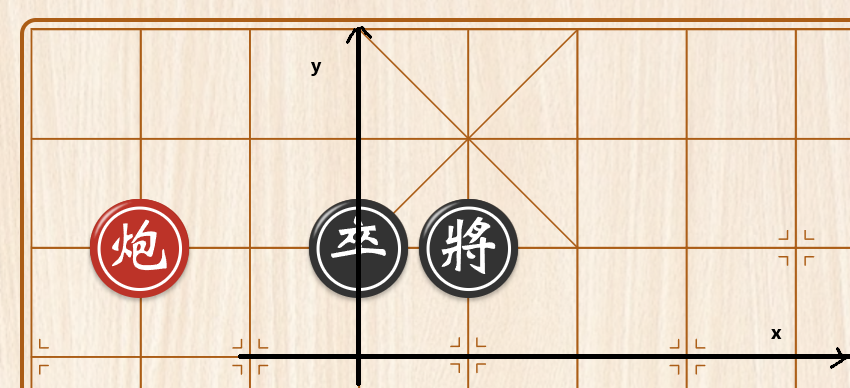
\includegraphics[scale = 0.5]{Problem_K_1.png}
   \caption{第 2 组测试数据的情况}
\end{figure}

下面的图展示了第 3 组测试数据的黑方棋子位置情况。

\begin{figure}[htbp]
   \centering
   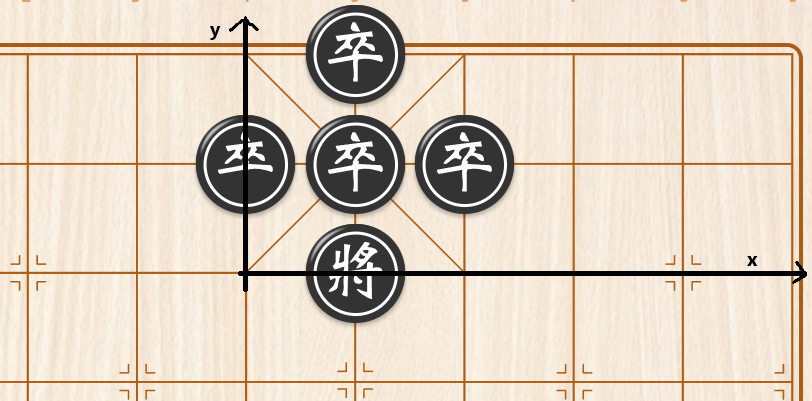
\includegraphics[scale = 0.5]{Problem_K_2.png}
   \caption{第 3 组测试数据的情况}
\end{figure}

请注意，为演示方便，示例图上画出了棋盘边界，但事实上题目描述中已经指出棋盘是无限大的。
\newpage
\section[L. 海底捞月]{\myboxxii{      \BF{\TT{L}}} 海底捞月}

\textit{运行时间限制}   2 seconds

\textit{内存使用限制} 1 Gigabyte

\textit{读入文件} \qquad 标准输入

\textit{输出文件} \qquad 标准输出


\begin{quote}
	\textit{\_\_\_, \_\_\_ 面色一沉：河底捞鱼是什么意思？}
\end{quote}

\subsection{题目描述}

TSUCE 的期末考试结束了！阅卷老师大 K 看了看小 T 惨不忍睹的试卷。

因此他决定使用以下的招数，拯救考了 $x$ 分的小 T：

\begin{itemize}
	\item 【连根拔起】，这个招数至多可以使用 $a_1$ 次，将小 T 当前的分数 $x$ 开根号乘 10 下取整，也即 $x \leftarrow \lfloor 10 \sqrt{x} \rfloor$.
	\item 【三七分成】，这个招数至多可以使用 $a_2$ 次，将小 T 当前的分数 $x$ 乘上 $0.7$ 再加上 30 再下取整， 也即 $x \leftarrow \lfloor 0.7x + 30 \rfloor$.
	\item 【种五得六】，这个招数至多可以使用 $a_3$ 次，将小 T 当前的分数 $x$ 乘上 $1.2$ 再 下取整，也即 $x \leftarrow \lfloor 1.2x \rfloor$.
	\item 【五福临门】，这个招数至多可以使用 $a_4$ 次，将小 T 当前的分数 $x$ 加 $5$，也即 $x \leftarrow x + 5$.
\end{itemize}

四种招数可以按任意顺序使用，请帮大 K 求出一个合理的使用招数的方式，来让小 T 获得最高的分数。

\subsection{输入格式}

第一行输入一个整数 $T$ ($1 \le T \le 3 \times 10^5$), 表示测试数据的数量。

每组测试数据输入一行 5 个整数 $x$, $a_1$, $a_2$, $a_3$, $a_4$ ($1 \le x \le 100, 0 \le a_1, a_2, a_3, a_4 \le 400$), 表示小 T 的初始分数，以及四种招数的可用次数上限。

\subsection{输出格式}

对于每组测试数据，输出一行一个整数表示小 T 可以获得的最高分数。

\subsection{样例 1}

\begin{minipage}{\linewidth}
	\begin{minipage}[t]{0.49\linewidth}
		\begin{lstlisting}[title=\texttt{standard input}]
7
1 1 1 1 1
50 2 1 1 2
99 0 1 2 1
10 2 0 0 3
100 400 400 400 400
75 1 7 3 0
1 3 7 4 3
\end{lstlisting}
	\end{minipage}
	\begin{minipage}[t]{0.49\linewidth}
		\begin{lstlisting}[title=\texttt{standard output}]
70
118
148
71
98703086085238798121046930830507710
168
232
\end{lstlisting}
	\end{minipage}
\end{minipage}


\subsection{样例 1 解释}

对于第 $1$ 组测试数据，小 T 一开始豪取 $1$ 分，大 K 每种招数都至多能使用一次，大 K 可以采用如下的策略：

\begin{itemize}
	\item 首先用 【三七分成】，小 T 变为 $\lfloor 0.7x+30 \rfloor = \lfloor 0.7 \times 1 +30 \rfloor = 30$ 分。
	\item 随后用 【连根拔起】，小 T 变为 $\lfloor 10\sqrt{x} \rfloor = \lfloor 10\sqrt{30} \rfloor = 54$ 分。
	\item 随后用 【五福临门】，小 T 变为 $54 + 5 = 59$ 分。
	\item 随后用 【种五得六】，小 T 变为 $\lfloor 1.2x \rfloor = \lfloor 1.2 \times 59 \rfloor = 70$ 分。
\end{itemize}

% \subsection{提示}

% 请选用合适的数据类型进行运算，样例 $1$ 种第 5 组数据的输出有 \[34 < \log_{10}(98\,703\,086\,085\,238\,798\,121\,046\,930\,830\,507\,710) < 35.\]





\newpage
\intentionalblankpage

\end{document}